\chapter{Contexte et problématique}

	\addcontentsline{toc}{section}{Introduction}
	\section*{Introduction}
	\lettrine{D}{ans} ce chapitre de la première partie, nous présentons l'entreprise où nous avons effectué notre stage académique à savoir ITS. Nous parlerons ensuite du contexte relatif à notre sujet de stage de fin d'étude, nous terminerons par une mise en évidence de la problématique lié à ce contexte  et les objectifs à atteindre. 
	

	%Presentation de l'entreprise
	\section{Présentation de l'entreprise}
		\subsection{Historique}
			ITS  est une entreprise spécialisée dans la protection des systèmes d'informations, la
sécurité informatique et la cryptologie de droit camerounais dont le siège générale se trouve à Yaoundé-Cameroun BP : 8570, plus précisément à Byem-Assi dans le $6^{ème}$ arrondissement du département de MFOUNDI. Elle commence ces services depuis 2008.
		
		\subsection{Organisation générale}
		
		
		\subsection{Missions}
			ITS est une entreprise résolument tournée vers l'innovation et en constante croissance. La mission d'ITS est de fournir à toute les entreprises et organismes publics, quelle que soit leur taille, les solutions des outils cryptographiques, de sécurité réseaux et de sécurités de systèmes d'informations le plus performant du marché. ITS fondé en 2008, est une entreprise leader dans le domaine de cryptographie et de sécurité des systèmes d'informations au Cameroun. Les solutions apportées par ITS permettent à leurs clients d'avoir l'assurance qu'une faille de sécurité ne menacera  jamais leurs activités. Ils peuvent donc consacrer totalement à leur croissance, car ces solutions les protègent efficacement contre les risques et les menaces informatiques. 
			D'ailleurs	sa réputation tient à la qualité des solutions de sécurités qu'elle met en place depuis sa création. Celles-ci intègrent les fonctionnalités essentiels suivantes :
			\begin{itemize}
				\item prévention d'intrusion (IDS),
				\item par-feu,
				\item protection antivirale et antispware,
				\item filtrage antispam et de contenu,
				\item PKI (Public Key Infrastructure),
				\item mobilité sécurité VPN,
				\item outils cryptographiques,
				\item etc.
			\end{itemize}
			Et enfin elle édifie les personnels des entreprises à travers de conférences, séminaires et webinaires et forme les intéressés dans plusieurs domaine de la sécurité informatique en vue de l'obtention de certificat à la fin de chaque formation.
		\subsection{Services et Produits}
			Entreprise ITS renferme plusieurs services, E-services et une centre de formations:
				\subsubsection{Sévices}
					Les services sont :
						\begin{itemize}
							  \item \textbf{Sécurité des SI :} Aujourd'hui l’implémentation des technologies de l'information et de la communication engendre les problèmes de types nouveaux de sécurité des informations sensibles,des infrastructures et organisations mises en place. Ainsi le contrôle et la gestion du risque informationnel dans ces nouveaux systèmes deviennent indispensables pour le bon fonctionnement et même l’existence de ces derniers. 
       						  \item \textbf{Investigation Numériques :}La cybercriminalité gagne du terrain avec la globalisation des systèmes d’information et l’intensification de leur utilisation dans tous les domaines d’activités de l’homme. La coopération internationale ne promet pas de résultats intéressants en même temps que les cybercriminels exploitent de mieux en mieux les technologies d’attaques disponibles, et ceci dans des conditions de partage d’expériences très bonnes. La police et les services de sécurité traînent le pas même si la législation permettant de combattre le fléau prend corps. La loi ne peut être efficace que si la preuve numérique du crime commis est à la disposition de la justice.
       						  \item \textbf{Audit des SI :}L’utilisation des systèmes d’information de plus en plus complexes et leur implémentation dans le contrôle et la gestion des processus sensibles imposent une normalisation visant la conformité de tous les systèmes d’information selon l’activité et le métier dans le but de mieux maitriser le risque qu’engendre le système d’information dans le fonctionnement de toute organisation. Ainsi l’audit des systèmes d’information comme activité visant a mesurer le niveau de conformité d’un système d’information par rapport a des règles bien définies et a examiner le niveau de dérive du système par rapport a ces standards aide a anticiper sur les problèmes et a proposer les solutions pour y remédier avant même l’occurrence d’incidents.
     						  \item \textbf{Gouvernance des SI :}Toute activité nécessite un système de gouvernance solide et efficace pour s’assurer de la pérennité de cette dernière, ainsi que de l’atteinte des objectifs fixe au départ. Le système d’information ne s’aurait faire exception à cette règle, au contraire nécessite plus d’attention dans ce sens car complexe et indispensable pour toute entreprise. Les investissements fais pour son système d’information doivent se justifier non pas par un besoin simple, mais au moyen d’une étude préalable présentant le gain retour sur cet investissement par la création et l’exploitation des services lies à l’investissement en question.
						\end{itemize}
				\subsubsection{E-Services}
					Dans les e-services on a plusieurs catégories :
					\begin{enumerate}
						\item \textbf{Web conférences:} rencontre internationale de Yaoundé sur la gestion du secret, l'usage de la cryptographie (Science du secret) dans la protection de l'information stratégique, la maîtrise des méthodes, moyens et systèmes de protection de l'information.
						\item \textbf{Web séminaires}
							\begin{itemize}
								\item \textbf{webinaire\footnote{Webinaire est un mot-valise associant les mots web et séminaire, créé pour désigner toutes les formes de réunions interactives de type séminaire faites via internet généralement dans un but de travail collaboratif ou d'enseignement à distance} Protection d'informations stratégiques :} Cette formation a pour objectif, la maîtrise des techniques de sécurisation et protection des informations stratégiques, ainsi que l'étude des mécanisme de protection de donnés sensibles.
								\item \textbf{webinaire : Audit informatique :} Le but de la formation est la maîtrise des notions et techniques d'audit des systèmes d'information, ainsi que l'étude des cas selon une démarche spécifique.
							\end{itemize}
                		\item Web consultations
        				\item E-Catalogue
                
					\end{enumerate}
    
				\subsubsection{Formations}
					Le centre de formation ITS est un centre de formation de référence spécialise dans les modules de formation suivants:
					\begin{itemize}
						\item sécurité des système d'information;
						\item investigations numériques;
						\item audit des systèmes d'information;
						\item gouvernance des systèmes d'information;
						\item développement informatique;
						\item infographie.
					\end{itemize} 
        Les formations ont un cycle de douze mois soit neuf mois de cours et trois mois de pratique en entreprise. Le centre de formation CF-ITS est agrée par le MINEFOPE(Ministère de l'Emploi et de la Formation Professionnelle) et donc délivre les certificats de fin de formation conformément à la réglementation en vigueur. En marge des formation dans les salles. \\
        
         Le centre donne l'accès gratuit et illimité aux forums et discussions via le portail web linkedin(www.linkedin.com) avec un nombre illimité d'experts internationaux du domaine de la cybercriminalité, cybersécurité, et investigation numériques, gouvernance et audit des systèmes d'information.
         
        		\subsubsection{Certifications}
        		
        		ITS offre également des certifications suivants :
        			\begin{enumerate}
        				\item Certification Professionnelle Nationale (MINEFOP)
        					\begin{itemize}
        						\item Sécurité des systèmes d’Informations
								\item Investigations numériques
								\item Audit des systèmes d’information
								\item Gouvernance des systèmes d’information
        					\end{itemize}
                		\item Certification Professionnelle Internationale (ISACA)
                			\begin{itemize}
                				\item CISM - Certified Information Security Manager
								\item CISA - certified Information Systems Auditor
								\item CRISC - Certified in Risk and Information Systems Control
								\item CGEIT-Certified in Governance of Enterprise IT
                			\end{itemize}
                		\item Certification Professionnelle Internationale (CISCO)
        			\end{enumerate}
				
				\subsubsection{Produits}
					L'entreprise a mis à la disposition de tout le monde des logiciels gratuit, on peut citer entre autre les logiciels suivants :
					\begin{itemize}
						\item Utilitaire de désinstallation d'antivirus \textbf{AVAST},
						\item Logiciel de calcul de l'empreinte numérique des fichiers,
						\item Calcul du hash code des fichier par \textbf{MD5},
						\item Logiciel d'\textbf{EBIOS},
						\item Logiciel de stéganographie,
						\item \textbf{Ntop} - Logiciel de \textbf{monitoring} du réseau.
					\end{itemize}
					
					Et des logiciels payants :
					\begin{itemize}
						\item Logiciel de récupération de mots de passe,
						\item etc.
					\end{itemize}
			
		
		\subsection{Cadre de stage}
			On a effectué notre stage au sein de la direction général de l'entreprise, elle se trouve dans le quartier \textbf{Biyem-Assi} dans la ville de Yaoundé, département de MFOUNDI plus précisément situé en plein cœur du 6e arrondissement. Leur direction se trouve dans l'\textbf{Avenue Biyem-Assi} à côté de \textbf{Pharmacie Les Béatitudes}.\\
		
		%\begin{minipage}{\textwidth}
			\subsubsection{Situation géographique}
			La figure ci-dessous présente l’emplacement de notre lieu de stage réalisé grâce au service du géant Google  \textbf{Google Map}.
				\begin{figure}[h]
					\centering
					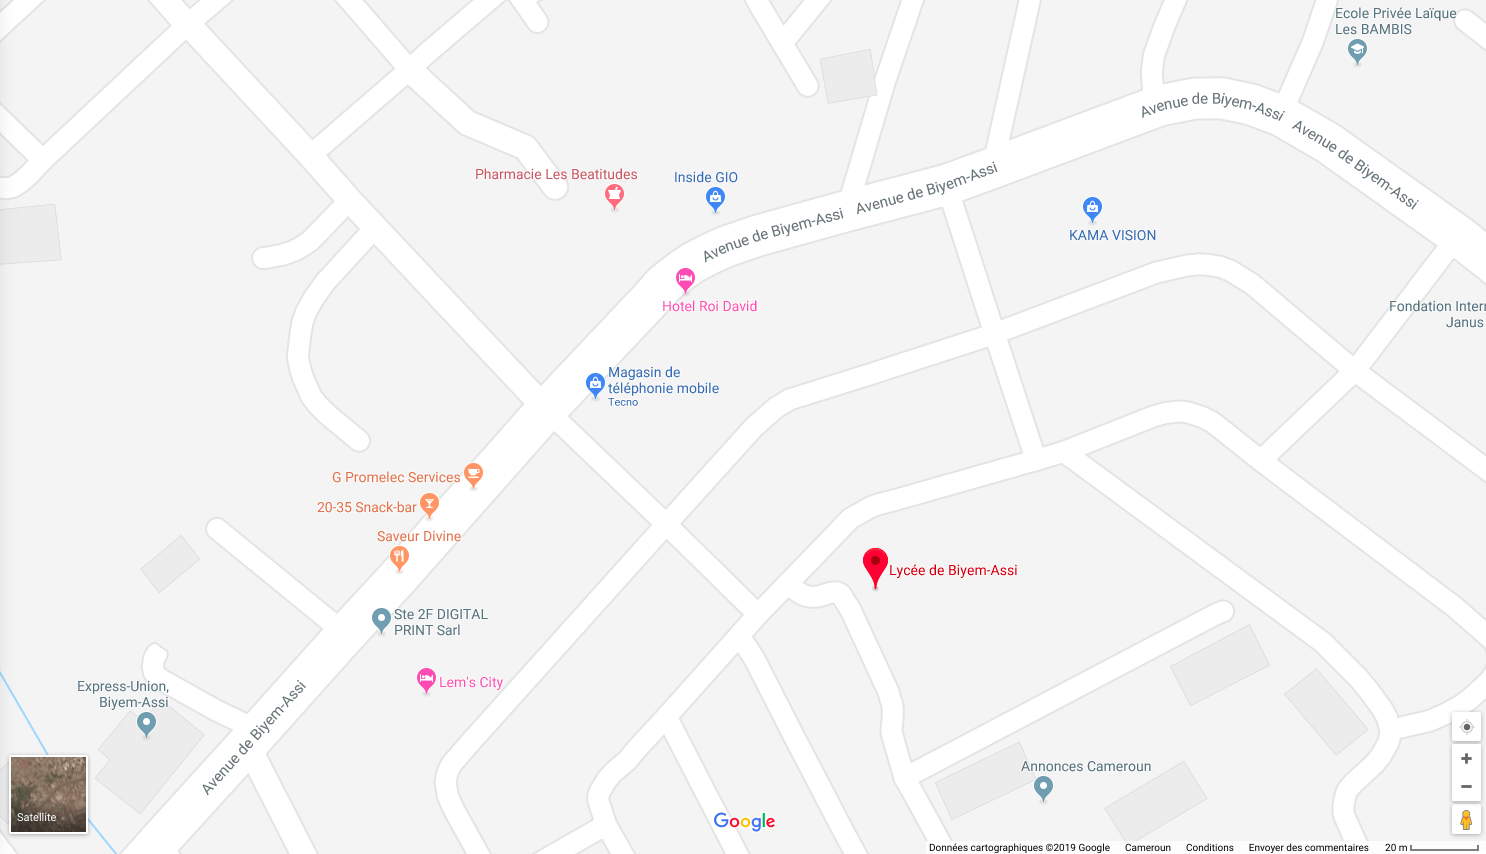
\includegraphics[scale=0.3]{../imgs/cartemap}
					\caption{Situation géographique du lieu de stage}
					\label{fig1}
			\end{figure}
		%\end{minipage}
			
	\section{Contexte}
		La création des signatures électroniques basé sur les infrastructures à clé publiques que sa soit avec OpenSSL ou d'autres se font soit en console, soit d'utiliser des outils propriétaires tels que :
		\begin{itemize}
			\item Word pour Microsoft,
			\item Adobe Reader de l'entreprise Adobe,
			\item DocuSign,
			\item Eversign,
			\item Yousign,\\
		\end{itemize}
		
		soit d'aller chez une Autorité de Certification (AC) pour générer un certificat, qui sont complexes et coûteux pour les utilisateurs et surtout à ceux qui débutent en développement des applications et en sécurité informatique. Et encore malheureusement ils sont déjà intégrés dans leurs applications complètes, donc pas des moyens de les réutiliser dans  d'autres logiciels comme des modules.\\
		
		Par ailleurs d'autres ne sont pas dans les systèmes d'exploitation libre(open source) comme Linux, par exemple \textbf{Word} de Microsoft et \textbf{Adobe Reader }ne fonctionnent pas sous Linux. 
	
	\section{Problématique}
			Les problèmes qui surviennent souvent dans les entreprises en particulier et chez les développeurs en général c'est la disposition des programmes modulaires pour intégrer facilement dans leurs plates-formes en fin de gagner en temps et en l'argent (surtout pour les entreprises). Ces nécessités nous amènent à nous poser les questions suivantes:\\
		
	\begin{itemize}
		\item Comment peut-on rendre cette difficulté de signer un document de manière transparente?
		\item Comment faciliter le développement d'un outil informatique au sein de l'entreprise ?
		
		\item Comment développer un module multi-plateforme ?
	\end{itemize}
	
	
	\section{Objectifs}
	
		\subsection{Objectif général}
			L'objectif principal de notre projet est d'offrir à l'entreprise et toute personne désirant signer un document électroniquement, un outil de signature électronique modulable. 
		
		\subsection{Objectif spécifique}
			De façon spécifique, il sera question pour moi de gérer les problèmes spécifiques liés aux :
			\begin{itemize}
				\item Création d'une signature des documents numériques (texte, son, vidéo, PDF, etc.) en se basant sur les infrastructures à clé publique ou PKI,
				\item automatisation de la création des signatures numériques,
				\item vérification de la signature de document numérique,
				\item prouver l'authenticité d'un signataire,
				\item faciliter à l'entreprise lors d'un besoin d'un module de signature électronique,
				\item génération des clés et chiffrement/déchiffrement des données,
			
				\item rendre la vie facile au développeur qui ne maîtrise pas forcément  la notion de cryptographie qui se cache derrière la signature numérique, d'intégrer ce module dans son plate-forme.\\
				%\item  
			\end{itemize}
			Ainsi les utilisateur avertis pourront juste l'importer dans leurs programmes et l'utilisé facilement. Tout ce qu'un utilisateur doit connaître c'est le nom de la méthode qu'il veut appeler avec sa signature (les paramètres de la méthode) et la méthode retournera le résultat voulu. Il y'aura une commande d'aide si l'utilisateur ne connais pas le nom de la méthode  avec sa signature(paramètre) et une manuelle bien documenté avec des exemples d'utilisations.	
			
		
	\section{Méthodologie}
		Pour atteindre ces objectifs, nous proposons à l'entreprise la conception et le déploiement d'un module de signature électronique basé sur l'infrastructure à clé publique (PKI). Nous allons suivre le cheminement de la conception dont  les grandes étapes sont suivantes :
		\begin{enumerate}
			\item  L’analyse des besoins du client qui débouchera sur l’élaboration d’un cahier de charges;
			\item  La conception du système qui débouchera sur la modélisation des différentes vues du système ;
			\item  L’implémentation logicielle qui est le codage proprement dit des différents éléments du système ;
			\item  Et enfin nous procéderons au déploiement, aux tests et validation.
		\end{enumerate}
	%\addcontentsline{toc}{section}{Conclusion}
	\section*{Conclusion}
		Dans ce chapitre de la première partie nous avons présenté le contexte et la problématique liés à notre thème et les services et produits que proposent ITS. En énumérant les problèmes que rencontre l'entreprise, les développeurs et les usagés lors de la signature électronique des documents numérique que nous proposons de résoudre par la mise en place de la conception et déploiement d'un module de signature électronique en se basant sur la infrastructure à clé publique. Dans le chapitre suivant, nous présenterons les généralités liés à la signature électronique en particulier et la cryptographie en générale.
